% !TeX spellcheck = en_US
\documentclass[sigconf,nonacm]{acmart}
\usepackage{graphicx}
\settopmatter{printacmref=false}
\pagestyle{empty}
\AtBeginDocument{%
  \providecommand\BibTeX{{%
    \normalfont B\kern-0.5em{\scshape i\kern-0.25em b}\kern-0.8em\TeX}}}
\copyrightyear{2020}
\acmYear{2020}
\setcopyright{rightsretained}
\begin{document}
\title{Security, Privacy \& Explainability in Machine Learning}
\subtitle{Exercise 1: Record-Linkage Attack}
\author{Thomas Jirout}
\email{thomas.jirout@tuwien.ac.at}
\affiliation{Mat.Nr. 01525606}
\author{Helmuth Breitenfellner}
\email{helmuth.breitenfellner@student.tuwien.ac.at}
\affiliation{Mat.Nr. 08725866}
\begin{abstract}
In this task we have been working on record-linkage attack.
For this we chose the dataset DBLP-Scholar provided by the University of Leipzig \cite{DataSets},\cite{kopcke2010evaluation}
and used the Python Record Linkage Toolkit \cite{de_bruin_j_2019_3559043}.

This report summarizes the identification of sensitive attributes, attributes
used for linking, and the performance of the record-linkage attack.
\end{abstract}
\keywords{Security, Privacy, Machine Learning, Record Linkage, Python}
\maketitle
\section{Task description and Fundamentals}

When performing a record linkage attack, there are a couple of steps
to be done:
\begin{itemize}
\item Acquire datasets
\item Cleanup \& pre-process data
\item Identify candidate pairs for linkage
\item Calculate matches on field-levels
\item Classify linked records
\item Evaluate classification
\end{itemize}

\subsection{Acquire datasets}

We were using the evaluation datasets, provided by the University Leipzig.
These datasets are already harmonized, i.e. the columns have the same names,
and there is also a set of ``ground truth'' linkage information
which we were using for the evaluation.

\subsection{Cleanup \& pre-processing}

Datasets contain errors: wrongly encoded strings, typos, or
incorrect years.
The purpose of the cleanup step is to reduce the influence of these
errors.
Approaches available include:
\begin{itemize}
\item Fuzzy text encoding, e.g. ``soundex'' code
\item Harmonization, e.g. lowercase of all text, removal of non-text characters
\end{itemize}

\subsection{Identify candidate pairs}

For performing a record linkage attack, one would have to compare each
record of the first with each record of the second dataset.
This becomes quickly infeasible once datasets reach hundred thousands
of records.

One approach to reduce this effort is using ``blocking''.
Here attributes are looked for which \emph{have} to agree for a
match to be considered.
Possible choice could be years where the errors are assumed to be
less prominent.

A variant of blocking is using a neighborhood. Instead of only
considering candidates with the same value one allows a small
difference of the values between the datasets.

Both blocking and neighborhoods significantly reduce the number
of candidate pairs to be inspected.

\subsection{Calculate matches on field-level}

For comparing strings there are multiple methods to gather a measure
of similarity supported by the Record Linkage Toolkit.
\begin{description}
\item[Levenshtein:]
The Levenshtein distance \cite{Levenshtein}
represents the number of edits required to change
from one to the other string.
\item[Damerau-Levenshtein:]
This is an enhancement suggested by Damerau \cite{Damerau} which
added an operation (transpose) to the set of possible edits.
\item[Jaro:]
The Jaro distance \cite{Jaro} gives a floating point value
in the interval [0,1] where 0 represents complete dissimilarity and 1
represents identical strings.
\item[Jaro-Winkler:]
This is an improvement on the Jaro distance described by Winker \cite{Winkler}
which also favors matches of longer common prefixes.
\item[Q-gram:]
This is an approximation for the Damerau-Levenshtein distance
described by Ukkonen \cite{Ukkonen}
which is quicker to calculate.
\item[Cosine:]
This is the usual cosine similarity, applied on the characters of
the strings.
\item[Smith-Waterman:]
This algorithm \cite{Smith-Waterman}, originally designed for finding similarities in
chemical molecules, looks for long identical subsequences to identify the similarity
of two strings.
\end{description}

An alternative to using these algorithms is using a phonetic code in
the pre-processing like soundex and then only allowing exact matches.

\subsection{Classify linked records}

To find the matches is a classification problem: given the calculated features
of field similarity, is this pair a real match?

There are multiple approaches implemented in the recordlinkage toolkit.

Some of them are supervised approaches, like \emph{Logistic Regression},
\emph{Naive Bayes}, \emph{Support Vector Machine}.
These approaches need a training phase to get the best parameters for
the classification.

Others are unsupervised, like \emph{KMeans Clustering} or
\emph{Expectation / Conditional Maximization}.

We created a \emph{train} dataset of about 20\% of the data to train
the supervised algorithms.
For comparability all algorithms (including the unsupervised ones)
were evaluated on the disjoint \emph{test} dataset.

\subsection{Evaluate}

There are multiple metrics for evaluating the quality of the classification.

We opted for metrics which do not count the number of pairs, as we felt
this is limiting in the results.
Therefore we opted for using the F1 score when looking at the quality
of the record linkage.

\section{Datasets}

For our record linkage experiments, we used the DBLP and Google Scholar evaluation datasets, provided by the University of Leipzig \cite{DataSets},\cite{kopcke2010evaluation}:

\begin{description}
\item[DBLP:] Publication records from the Digital Bibliography \& Library Project, consisting of 2616 records.
\item[Scholar:] Publication records from Google Scholar, consisting of 64263 records.
\item[Perfect Mapping:] Along with the DBLP and Scholar datasets, the University of Leipzig also provided a ``perfect mapping'', which we used in our evaluation step to determine the quality of our record linkage results. According to this perfect mapping, a perfect record-linkage attack would be able to find 5348 id-to-id matches. It is worth noting that it can be seen from this document that assignments are m-to-n, meaning that it is possible that any entry in one dataset may correspond to multiple entries in the other one.
\end{description}

These datasets were already harmonized, i.e. the columns had the same names: id (string), title of the publication (string), authors (string), publication venue (string or NULL) and year (integer or NULL).

\subsection{Data Linking}

Due to the nature of the ready-prepared dataset, the identification of the
linked attributes was very easy.

We used the following attributes to link records:
\textbf{Name} (of the publication), \textbf{Venue} and \textbf{Authors}.

\subsection{Example Data}

As a demonstration of the difficulty of matching two entries, Table \ref{ExampleData} shows rows that would be a match, but are represented in a slightly different manner in each of the datasets.

\begin{table*}[th]
\begin{tabular}{|l|l|l|l|l|l|}
\hline
dataset & id & title                        & authors                                                                                                                                                                              & venue             & year \\ \hline
DBLP    &  journals/sigmod/SnodgrassAABC  & TSQL2 Language Specification & R Snodgrass, I Ahn, [...] & SIGMOD Record     & 1994 \\ \hline
Scholar &   64iWa-ZiPRcJ & TSQL2 language specification & RT Snodgrass                                                                                                                                                                         & ACM SIGMOD Record & 1994 \\ \hline
\end{tabular}
\caption{Example Data Entries from DBLP and Scholar Dataset (id and authors column abbreviated)}
\label{ExampleData}
\end{table*}

\subsection{Sensitive attributes}

Normally datasets of articles do not contain sensitive information,
and authors would like to have the contained data shared with
as many people as possible.

For the purpose of out evaluation we were qualifying the
ID on Google Scholar as sensitive.

The idea is that through these ID values more information
can potentially be revealed, e.g. citations of the authors.


\section{Evaluation \& Summary}

For our evaluation, we created a python script that iteratively
ran the configurations of our individual experiments and created
the required figures, making it easy for us to interpret and
compare the results.

\subsection{Impact of Preprocessing}

We were comparing the preprocessing impact on the F1 score of
the record linkage.
Since we expected a difference in whether we use a simple comparing
algorithm (like ``exact'' match) and a more complex one (like ``jaro'')
we run the various preprocessing options against these two comparison
alternatives.
The impact on the F1-score is shown in figure \ref{plot:preprocessing}.

\begin{figure}[h]
\centering
\caption{Impact of Preprocessing}
\label{plot:preprocessing}
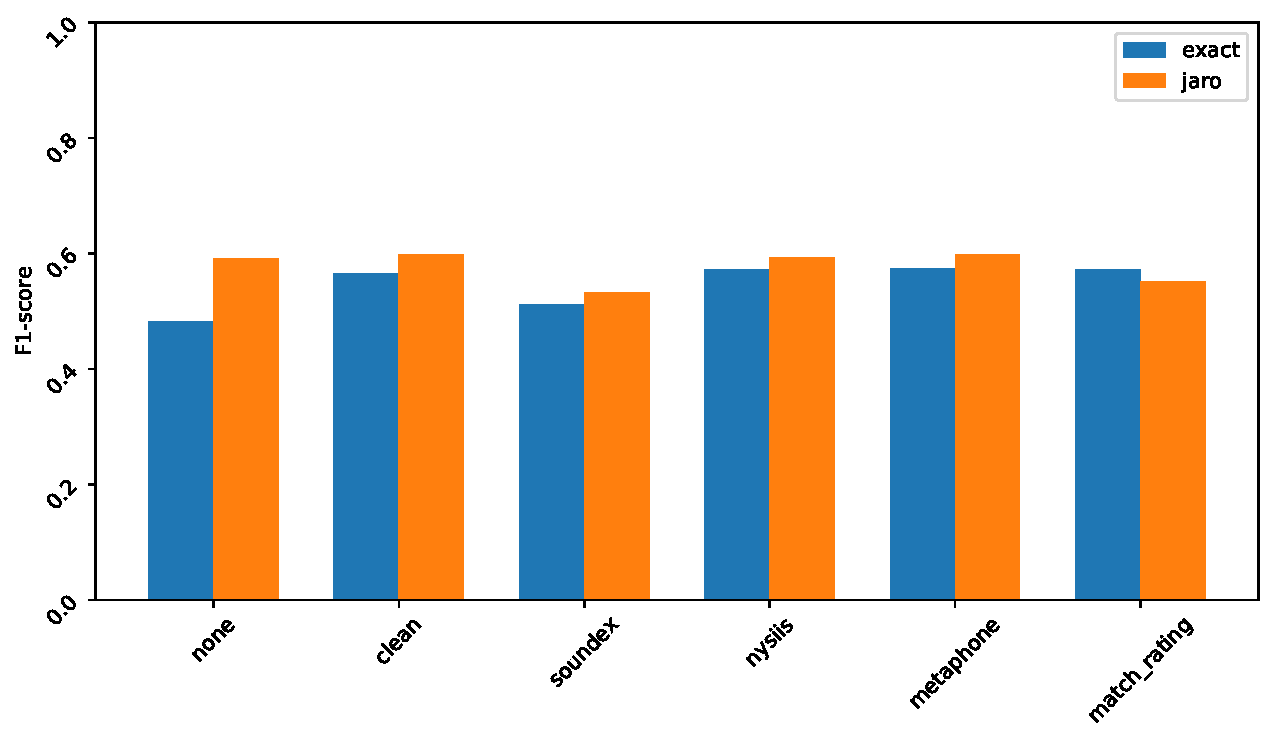
\includegraphics[width=0.9\linewidth]{../figures/eval_preprocessing}\\[-2mm]
\emph{\small
This graphic shows the impact of various preprocessing methods, in combination with both ``exact'' and ``jaro'' match, on the F1-score.
For the comparison a blocking index, together with an SVM classifier were used.}
\end{figure}

As is visible from the graph, no preprocessing \emph{at all} together
with a good comparing algorithm like ``jaro'' delivered comparable results
to cleaning.
Another observation is that \emph{exact} word match performs well when coupled
with a phonetic encoding - especially ``nysiis'' was quite powerful here.

\subsection{Impact of Indexing Step}

As part of this experiment, we compared different indexing methods
in terms of their impact on the linking result as well as the impact
they had on the processing time.

In particular, we compared different configurations of the indexer
called
\texttt{SortedNeighborhood}, using the ``year'' column
as the linking attribute. The impact on the quality of the
linkage (precision, recall and F1-score) are shown in figure \ref{plot:index}.
When comparing the performance of the different indexing techniques
(block index on the year, vs using a window) we see that the F1-score is hardly
affected, but the runtime is exploding.
This is an indication that the attribute year is accurately represented
in both datasets.
On the other hand, we can see that using a good indexing configuration
can have a major impact on the computation time of the following step
while still achieving satisfying linking results.

\begin{figure}
\centering
\caption{Impact of index on linkage quality}
\label{plot:index}
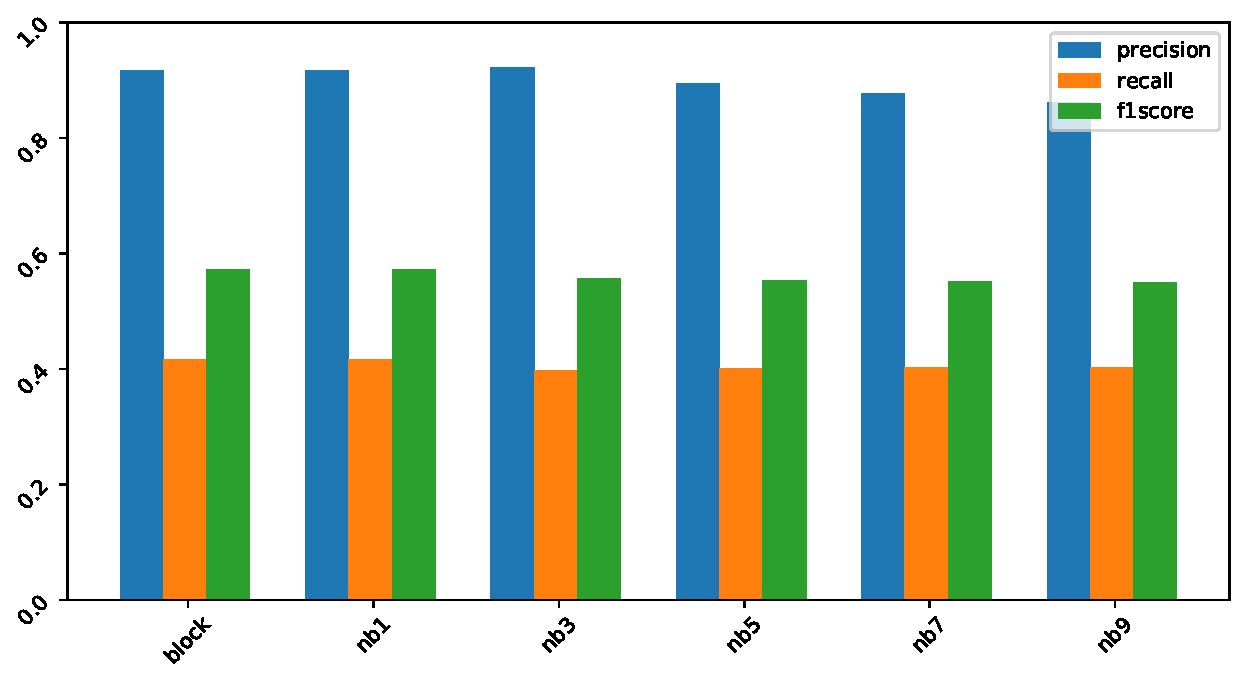
\includegraphics[width=0.9\linewidth]{../figures/eval_indexing}\\[-2mm]
\emph{\small This graphic shows the impact of the index strategy on the quality
of the linkage.
For performance reasons, a
Nysiis encoding together with exact matching was used.}
\end{figure}

\emph{Note the logarithmic scale on figure \ref{plot:index2}.}

\begin{figure}[h]
\centering
\caption{Impact of index on runtime}
\label{plot:index2}
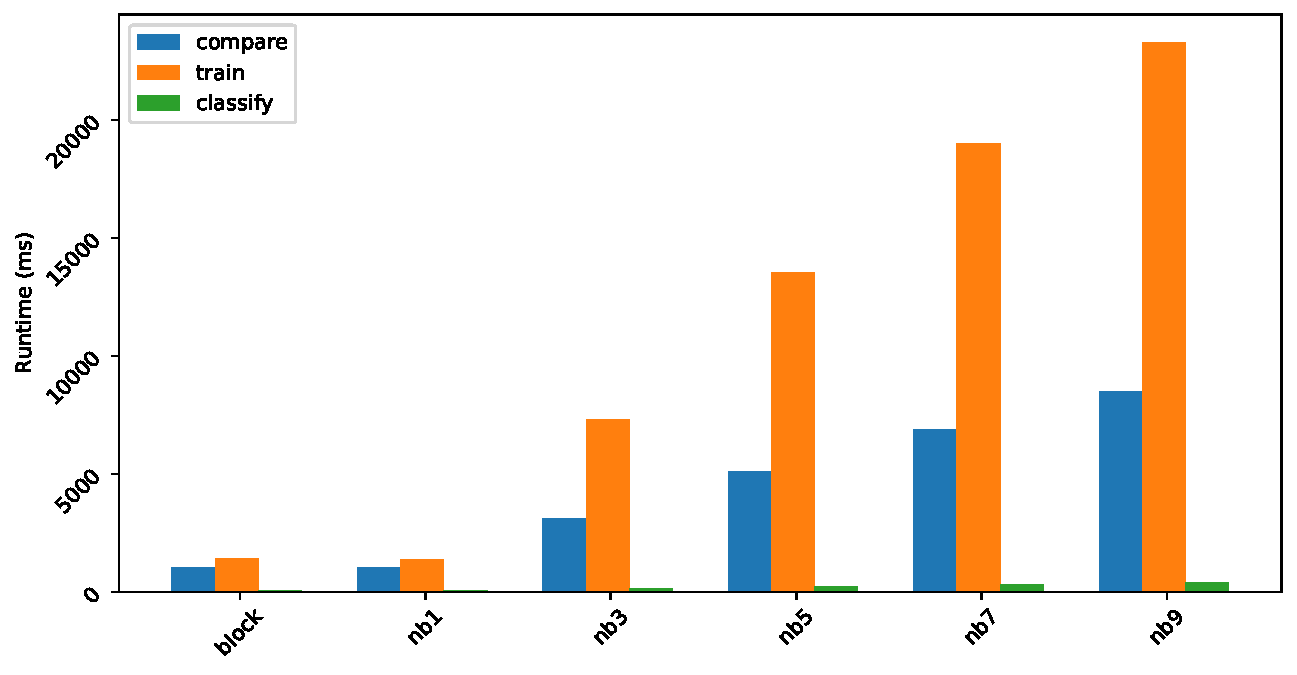
\includegraphics[width=0.9\linewidth]{../figures/eval_indexing2}\\[-2mm]
\emph{\small
This graphic shows the impact of index choice on the runtime of performing
a linkage attack.}
\end{figure}


\subsection{Impact of comparison methodology}

The comparison methods have some influence on the F1 score.
When running them against a fixed configuration (block index,
cleaning without phonetic encoding, and using logistic regression),
we saw that Exact, Levenshtein and Damerau-Levenshtein were performing best,
together with Q-Gram, Cosine similarity and Smith-Waterman.
See figure \ref{plot:comparison} for the results.

\begin{figure}[h]
\centering
\caption{Impact of comparison method on F1 score}
\label{plot:comparison}
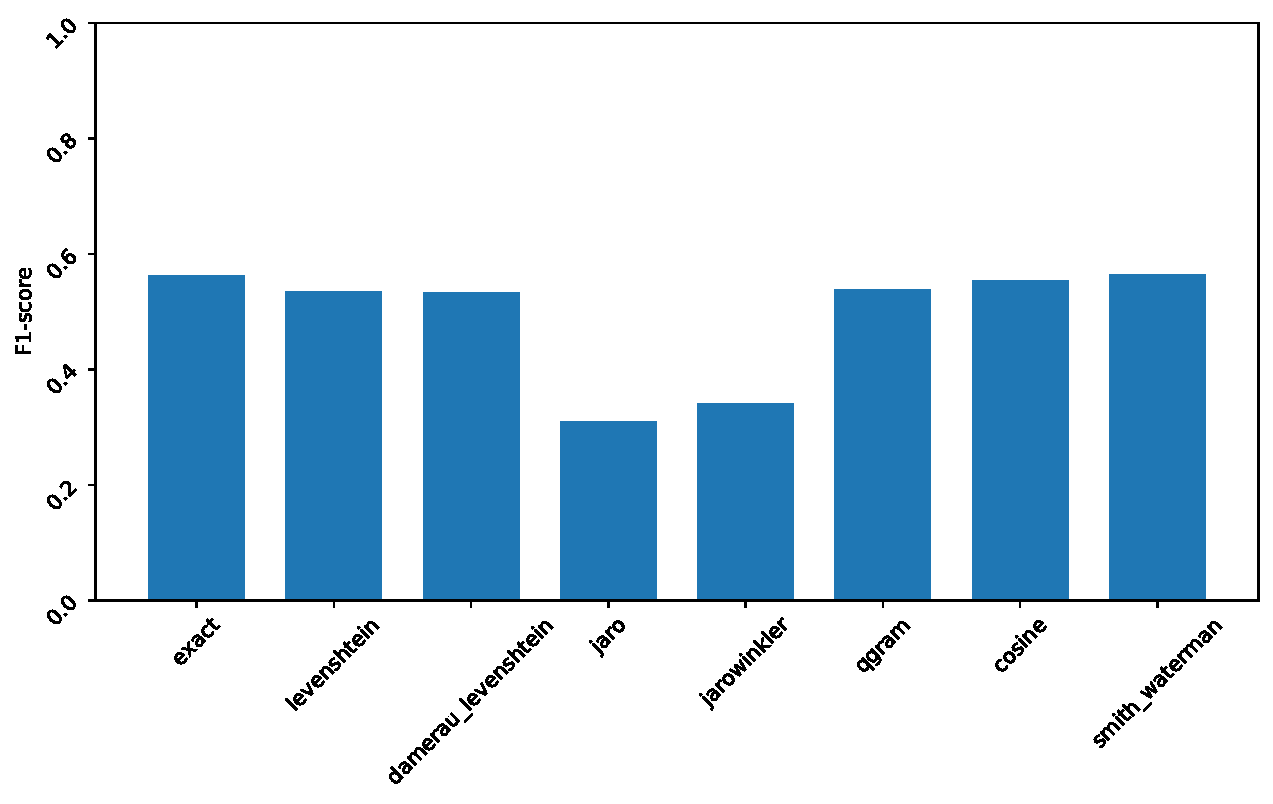
\includegraphics[width=0.9\linewidth]{../figures/debug_eval_comparison}\\[-2mm]
\emph{\small
This graphic shows the impact of the comparison algorithm on the
quality of the linkage, measure using F1 score.
Cleaning as preprocessing, a block index on the year,
and Logistic Regression were used for all values.}
\end{figure}

These results are however to be taken with some reservation, as these
graphs were created on a reduced set of about 10\% of the data, as otherwise
the runtime would not have been reasonable.

The general impact on the runtime is presumably representative despite the
smaller dataset.
As can be seen on figure \ref{plot:comparison2}, the runtime of Smith-Waterman
is more than 100 times larger than the runtime of Jaro or Jaro-Winkler
- \emph{and both are already more than 20 times slower than an exact match!}

\begin{figure}[h]
\centering
\caption{Impact of comparison method on runtime}
\label{plot:comparison2}
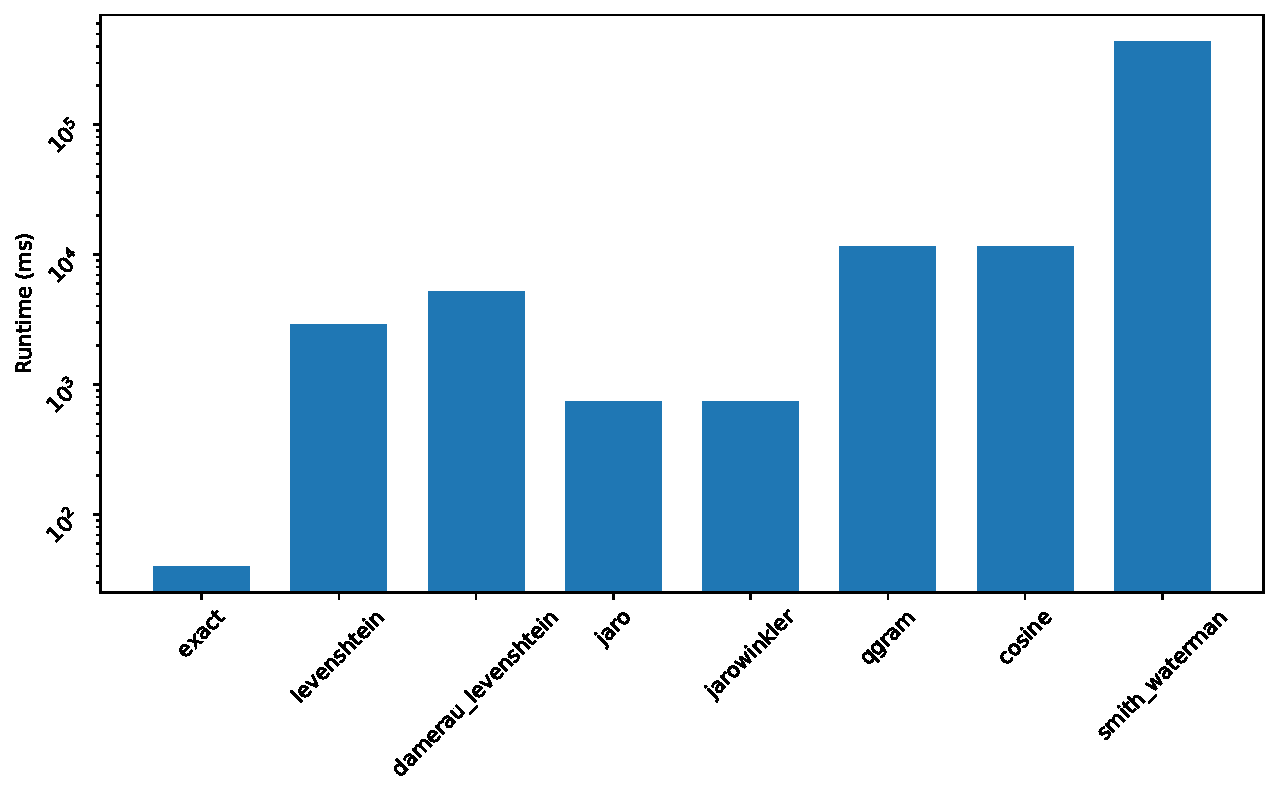
\includegraphics[width=0.9\linewidth]{../figures/debug_eval_comparison2}\\[-2mm]
\emph{\small
This graphic shows the impact of the comparison algorithm on the
runtime of the comparison step.
Cleaning as preprocessing and a block index on the year were used for all values.}
\end{figure}

\subsection{Impact of Classifier}

We were trying out all comparison methods implemented by default in the
\emph{recordlinkage} toolkit.
For two algorithms (Naive Bayesian, ECM) it is necessary to binarize
the attributes - we have chosen a threshold of 0.75 for this.
See figure \ref{plot:classifier} for the results.

We see that the KMeans algorithm is performing very poorly.
This was expected, as also the documentation of the recordlinkage toolkit
is stating that KMeans clustering is not the method of choice for record
linkage.

\begin{figure}[h]
\centering
\caption{Impact of classifier on linkage quality}
\label{plot:classifier}
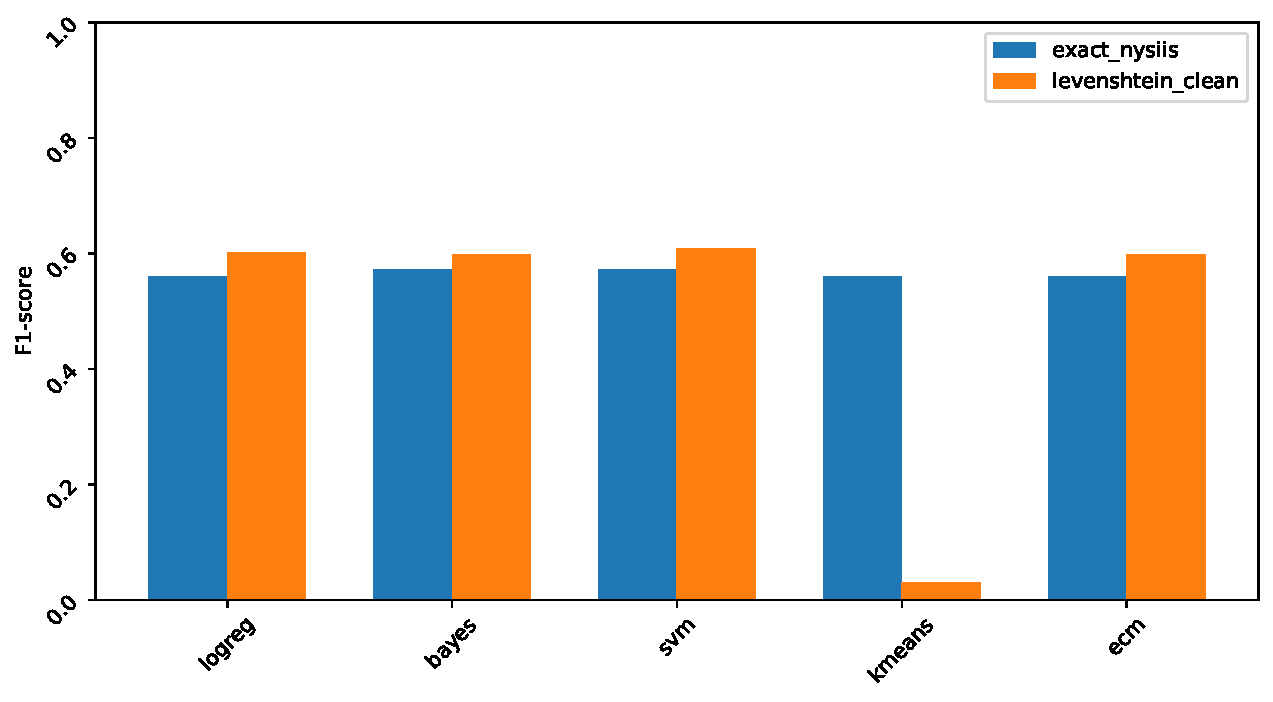
\includegraphics[width=0.9\linewidth]{../figures/eval_classifier}\\[-2mm]
\emph{\small
This graphic shows the impact of the classifier algorithm on the
quality of the linkage.
Two configurations were tested: phonetic Nysiis encoding with
exact match, and data cleaning with Levenshtein comparing.}
\end{figure}

The difference in the runtime of the classifiers is not so much
emphasized, as shown in figure \ref{plot:classifier2}.
Still the \emph{ECM} algorithm is by far the slowest one of the
offered algorithms.

\begin{figure}[h]
\centering
\caption{Impact of classifier on linkage quality}
\label{plot:classifier2}
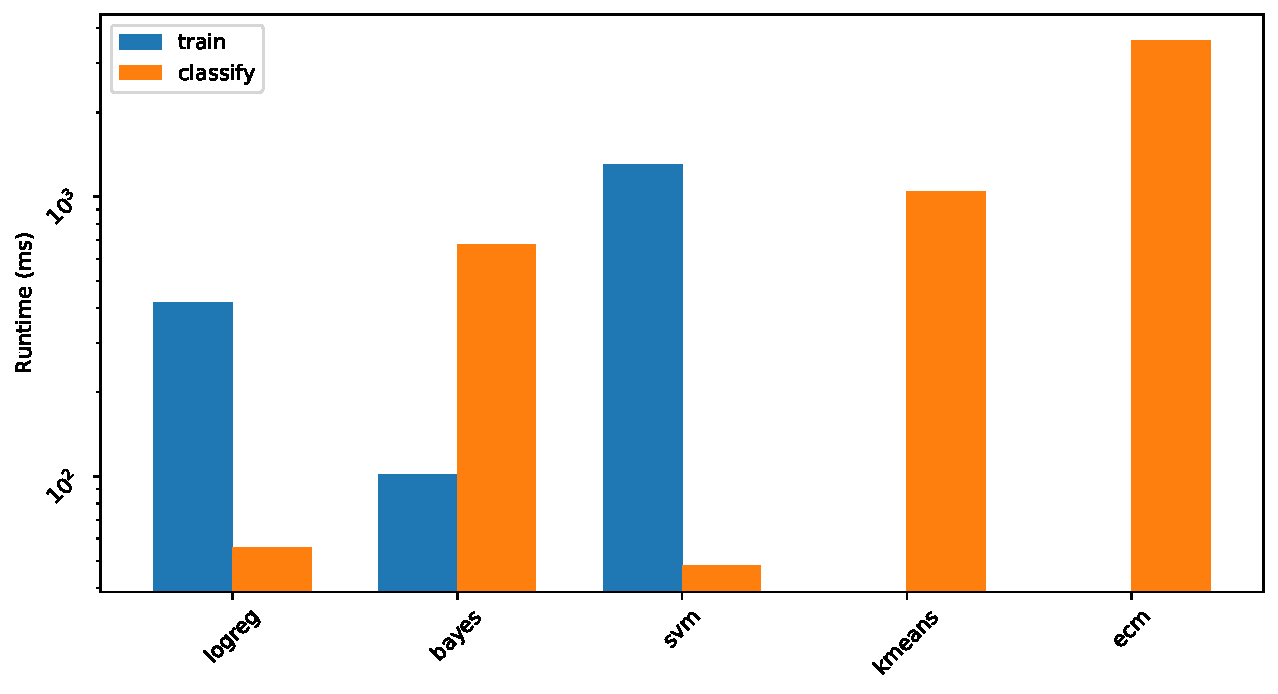
\includegraphics[width=0.9\linewidth]{../figures/eval_classifier2}\\[-2mm]
\emph{\small
This graphic shows the impact of the classifier algorithm on the
runtime of the classification steps (training and predicting).
For this comparison phonetic Nysiis encoding with
exact match were used.
Note that for most cases the runtime is mostly influenced by the compare step,
unless exact match is chosen.}
\end{figure}

\subsection{Summary}

Which combination would we choose when tasked to perform a real
record linkage?

This very much depends on the size of the datasets available.
For very large sets, using a good preprocessing like \emph{nysiis}
with a fast comparison like \emph{exact} seems like a good choice.

For performing the classification our favorite is \emph{Logistic Regression}
- its runtime is way better than the other algorithms when using on a
20\%-80\%
train-test split.
If the training dataset would be significantly smaller, then
\emph{SVM} is a good choice as it is even faster in doing the
classification after training.

And we would also focus on identifying possible blocking attributes,
if necessary by extracting subfeatures from the data.
Having a block index significantly reduces the runtime of doing the
record linkage.

Overall performing the linkage attack was quite interesting.
Only caveat is that the dataset we chose is of such high quality
and already prepared for record linkage, that the steps of
data cleaning, identification of linkage attributes and
also the search for quasi identifier and sensitive attributes
were not that present as we would expect in a real-world
case.

\bibliographystyle{ACM-Reference-Format}
\bibliography{report}
\end{document}
